\section{Task Description}
\label{sec:taskedes}
As previously said the robotic arm has to move along a predefined polygonal trajectory with the aim to cut surfaces which follows above it in a horizontal plane. The steps that manipulator performs in order to accomplish its objective are concerned as follows:

\begin{enumerate}[label=\roman{*}., ref=(\roman{*})]
	\item Every time begins a new instance of the task the robotic arm lies in a initial predefined pose, in such pose its $x$ and $y$ coordinates corresponds to the top-left corner of a rectangle, while its $z$ coordinate distances the cutting plane of a certain amount. Then it starts to moving across down direction.
	\item Once height of the laser tool reaches a reasonable cutting-height it stops to moving down and then follows the rectangular trajectory. When all sides of such rectangle are completed it lies again in the top-left corner, so it starts again to move up to reach the predefined pose and wait a new task instance.
\end{enumerate}

A graphical representation of the trajectory computed in one task instance is represented in Fig.\ref{fig:traj}

\begin{figure}[!h]
\centering
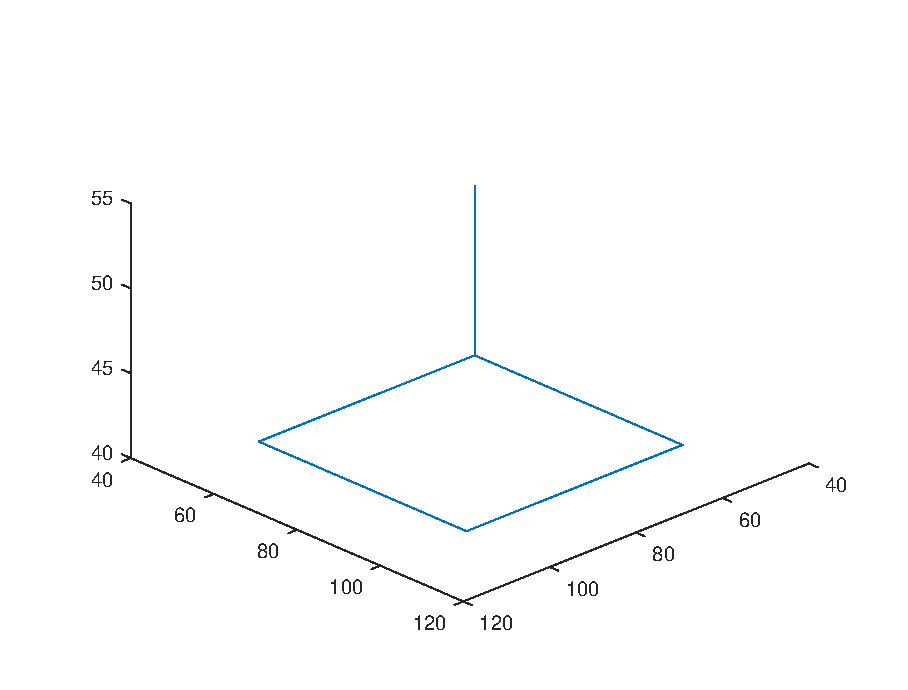
\includegraphics[width=1\linewidth]{img/traj}
\caption{Task trajectory}
\label{fig:traj}
\end{figure}
Which in terms of coordinates is
\begin{figure}[!h]
	\centering
	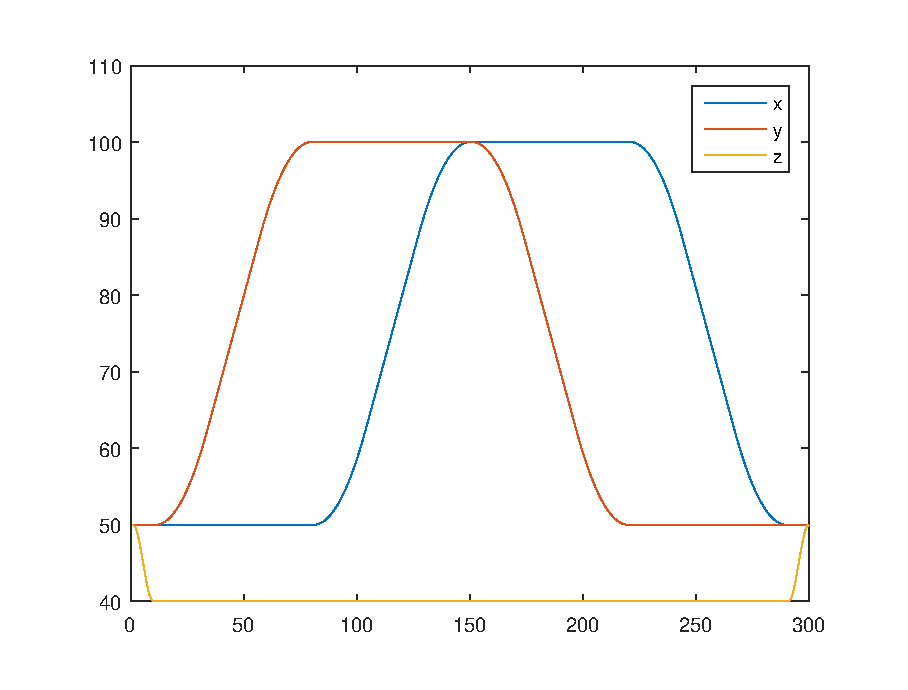
\includegraphics[width=\linewidth]{img/trajcoord}
	\caption{Task trajectory coordinates}
	\label{fig:trajc}
\end{figure}
\newpage
Each trajectory side has been generated in the Cartesian space by means of the \textit{ctraj} function of \textit{Robotics Toolbox}, which takes as inputs two homogeneous matrix, representing initial and final pose, and a vector representing the number of point for each segment of the generated trajectory.
Follows a stub of trajectory generation procedure:
\begin{center}
\begin{lstlisting}
function traj = rectraj(r, sps)
traj = zeros(4,4,sum(sps));
for i=1:7
t(:,:,i)= transl(r(i,:));
for j=1:6
if j==1
traj(:,:,1:sps(j)) = ctraj(t(:,:,j), t(:,:,j+1), sps(j)); 
else
traj(:,:,sum(sps(1:j-1))+1:sum(sps(1:j-1))+sps(j))=ctraj(t(:,:,j),t(:,:,j+1),sps(j)); 
end        
end
\end{lstlisting}
\end{center}
Where r is an array representing a collection of rectangle vertices plus the initial point. It is computed through another simple function:
\begin{center}
\begin{lstlisting}
  r = rect(tl_corner, width, height);
\end{lstlisting}
\end{center}
